%%% Lecture 6

\section{Proof of Hurewicz Theorem}

\lecture[Hurewicz theorem at last! Then some generalities about fibre bundles.]{2021-11-3}

\begin{proof}[Proof of the Hurewicz theorem (\ref{theorem:hurewicz})]
We modify the definition of $\pi_n(X,A)^\#$ by replacing $\pair$ by the homeomorphic pair $(\ns,\de\ns)$.

Then the fundamental class $i\in H_n(\ns,\de\ns;\Z)$ is represented by the map $\id_\ns\in\S(\ns)_n$. The inclusion of simplicial sets (the $\cong$ comes from theorem \ref{theorem:simplicial-deformation-retraction} of last lecture)
\[\S(A)\into\S(X,A,n-1)\xinto{\cong}\S(X)\]
induces morphisms of chain complexes
\[C(\S(A))\to C(\S(X,A,n-1))\xto{\sim}C(\S(X))\]
where \enquote{$\sim$} is a chain homotopy equivalence.

We compare the long exact homology sequences:
\begin{center}
    \small
    \begin{tikzcd}
    \cdots \arrow[r] & H_n(A) \arrow[d, eq] \arrow[r] & H_n(C(\S(X,A,n-1))) \arrow[d, "\cong"] \arrow[r] & H_n(\frac{C(\S(X,A,n-1))}{C(\S(A))}) \arrow[d,"\cong \text{ (by 5-lemma!)}"] \arrow[r,"\de"] & \cdots \\
    & H_n(A) \arrow[r] & H_n(X) \arrow[r] & H_n(\frac{C(\S(X))}{C(\S(A))})=H_n(X,A) \arrow[r, "\de"] & \cdots
    \end{tikzcd}
\end{center}

Conclusion: the inclusion $\S(X,A,n-1)\into\S(X)$ induces an isomorphism
\[H_n\left(\frac{C(\S(X,A,n-1))}{C(\S(A))}\right)\xto{\cong} H_n(X,A)\]
so that we reduced the problem to finding an isomorphism
\[\pi_n(X,A)^\#\xto{``\cong"} H_n\left(\frac{C(\S(X,A,n-1))}{C(\S(A))}\right)\]

We note that $\S(X,A,\ni)_\ni=\S(A)_\ni$ so
\[\left(\frac{C(\S(X,A,n-1))}{C(\S(A))}\right)_\ni=0\]
which implies
\begin{align*}
    H_n(X,A)&\cong H_n\left(\frac{C(\S(X,A,n-1))}{C(\S(A))}\right) \\
    &=\coker\left(\frac{\Z[\S(X,A,\ni)_{n+1}]}{\Z[\S(A)_{n+1}]}\xto{\quad d\quad} \frac{\Z[\S(X,A,\ni)_n]}{\Z[\S(A)_n]}\right) \\
    &=\Z[f:(\ns,\de\ns)\to (X,A)]/E''
\end{align*}
where $E''$ is the subgroup generated by:
\begin{itemize}[label={-}]
    \item the classes of all $f:(\ns,\de\ns)\to(X,A)$ with $f(\ns)\subset A$,
    \item elements of the form $\sum_0^{n+1}(-1)^id_i^*(g)$ for all $g:\sx{n+1}\to X$ with $g(\sk_\ni(\sx{n+1}))\subset A$.
\end{itemize}

On the other hand, $\pi_n(X,A)^\#=\Z[f:(\ns,\de\ns)\to\pairs]/E'$
where $E'$ is generated by:
\begin{itemize}[label={-}]
    \item $f-f'$ for all pair homotopic $f\sim f'$,
    \item $f_1+f_2-(f_1\oplus f_2)$ whenever $f_1$ and $f_2$ are "addible".
\end{itemize}

To add maps on simplices of the same dimension, we divide $\ns$ into two sub-simplices by a procedure defined inductively, using the hyperplane $T^n$ in $\ns$ through $e_0$ and the hyperplane $T^{n-1}$ dividing $d_0(\sx{n})$. Pictured below, the $n=2$ case, starting with $T^1=\sum \frac{1}{2} e_i$.
\begin{center}
    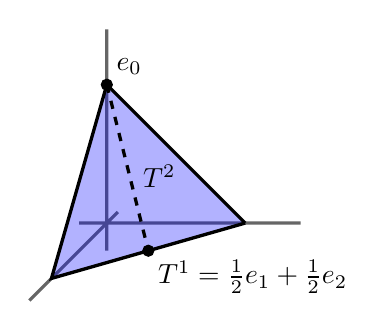
\begin{tikzpicture}[x=1em, y=1em, z=-0.4em, baseline=0.8em]
    \draw[very thick, black!60] 
        (-1,0,0) -- (7,0,0)
        (0,-1,0) -- (0,7,0)
        (0,0,-1) -- (0,0,7);
    \fill[fill=blue, opacity=0.3]
        (5,0,0)--(0,5,0)--(0,0,5)--(5,0,0);
    \draw[very thick, black]
        (5,0,0)--(0,5,0)--(0,0,5)--(5,0,0);
    \draw[dashed, very thick] (0,5,0) -- (2.5,0,2.5);
    \filldraw 
        (0,5,0) circle (2pt) node[anchor=south west] {$e_0$}
        (2,3.5,2.6) node[anchor=north west] {$T^2$}
        (2.5,0,2.5) circle (2pt) node[anchor=north west] {$T^1=\frac{1}{2}e_1+\frac{1}{2}e_2$};
    \end{tikzpicture}$\quad\quad\quad\quad$
    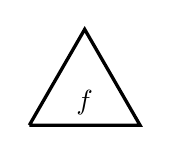
\begin{tikzpicture}[x=4em, y=4em, baseline=0.8em]
    \draw[very thick] (0,0) -- (1,0) -- (0.5, 0.866) -- (0,0);
    \filldraw (0.5, 0.2) node {$f$};
    \end{tikzpicture}$+$
    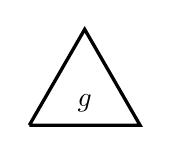
\begin{tikzpicture}[x=4em, y=4em, baseline=0.8em]
    \draw[very thick] (0,0) -- (1,0) -- (0.5, 0.866) -- (0,0);
    \filldraw (0.5, 0.2) node {$g$};
    \end{tikzpicture} $=$
    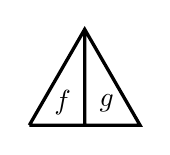
\begin{tikzpicture}[x=4em, y=4em, baseline=0.8em]
    \draw[very thick] (0,0) -- (1,0) -- (0.5, 0.866) -- (0,0)
    (0.5,0)--(0.5, 0.866);
    \filldraw (0.3, 0.2) node {$f$}
    (0.7, 0.2) node {$g$};
    \end{tikzpicture}
\end{center}

Claim. The canonical homomorphism
\[\Z[f:(\ns,\de\ns)\to\pairs]\to \pi_n\pairs^\#,\quad [f]\mapsto[f]\]
factors through a homomorphism
\[\Phi: H_n\left(\frac{C(\S(X,A,n-1))}{C(\S(A))}\right)\to\pi_n\pairs^\#\]
(which is equivalent to saying that $E''\subset E'$).

\begin{claimproof}
We need to show that the two kinds of relations that generate $E''$ are sent to $0$.
\begin{itemize}[label={-}]
    \item If $f:(\ns,\de\ns)\to\pairs$ has image in $A$, we contract $\ns$ onto $e_0$ and postcompose this contraction homotopy with $f$. The result is a pair homotopy from $f$ to a constant map with value $f(e_0)$. So $[f]=[\const_{f(e_0)}]$, which is the zero element in $\pi_n\pairs^\#$.
    \item Now we consider all maps $g:\sx{n+1}\to X$ with $g(\sk_\ni(\sx{n+1}))\subset A$. We want to show that $\sum_0^{n+1}(-1)^i [g\circ(d_i)_*]=0$ in $\pi_n\pairs^\#$.
\end{itemize}

We consider the space $B=\sx{n}\cup_{\sx{n-1}}\dots\cup_{\sx{n-1}}\sx{n}$. It is a quotient space of a disjoint union of $n+2$ copies of $\ns$. If we number these copies from $0$ to $n+1$, we glue the $i$-th copy to the $(i+1)$-st copy by the maps:
\begin{center}
    \begin{tikzcd}
    \sx{\ni} \arrow[d,"(d_i)_*"] \arrow[r,"(d_i)_*"] & \ns_{((i+1)\text{-st})} \\
    \ns_{(i\text{-th})}
    \end{tikzcd}
\end{center}

Informally, $B$ is $\de\sx{n+1}$ "cut open", as shown in the following picture.
\begin{center}
    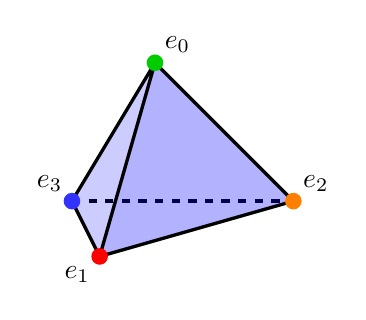
\begin{tikzpicture}[x=1em, y=1em, z=-0.4em, baseline=0.8em]
    \draw[very thick, black, dashed] 
        (-3,0,0) -- (5,0,0);
    \fill[fill=blue, opacity=0.3]
        (5,0,0)--(0,5,0)--(0,0,5)--(5,0,0);
    \fill[fill=blue, opacity=0.2]
        (-3,0,0)--(0,5,0)--(0,0,5)--(-3,0,0);
    \draw[very thick, black]
        (5,0,0)--(0,5,0)
        (0,0,5)--(5,0,0)
        (0,5,0)--(0,0,5)
        (-3,0,0)--(0,5,0)
        (0,0,5)--(-3,0,0);
    \filldraw 
        (0,5,0) circle (2pt) node[anchor=south west] {$e_0$}
        (5,0,0) circle (2pt) node[anchor=south west] {$e_2$}
        (0,0,5) circle (2pt) node[anchor=north east] {$e_1$}
        (-3,0,0) circle (2pt) node[anchor=south east] {$e_3$};
    \fill[red]
        (0,0,5) circle (3pt);
    \fill[blue!80]
        (-3,0,0) circle (3pt);
    \fill[green!80!black]
        (0,5,0) circle (3pt);
    \fill[orange]
        (5,0,0) circle (3pt);
    \end{tikzpicture}$\quad\quad\quad\quad$
    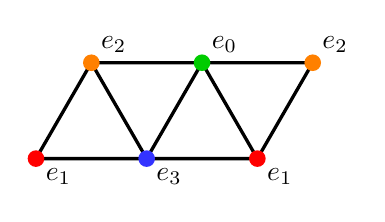
\begin{tikzpicture}[x=4em, y=4em, baseline=0.8em]
    \draw[very thick]
        (0,0) -- (2,0)
        (0,0) -- (0.5, 0.866)
        (1,0) -- (0.5, 0.866)
        (0.5, 0.866) -- (2.5, 0.866)
        (1,0) -- (1.5, 0.866)
        (2,0) -- (1.5, 0.866)
        (2,0) -- (2.5, 0.866);
    \filldraw
        (0,0) node[anchor=north west] {$e_1$}
        (1,0) node[anchor=north west] {$e_3$}
        (2,0) node[anchor=north west] {$e_1$}
        (0.5, 0.866) node[anchor=south west] {$e_2$}
        (1.5, 0.866) node[anchor=south west] {$e_0$}
        (2.5, 0.866) node[anchor=south west] {$e_2$};
    \fill[red]
        (0,0) circle (3pt)
        (2,0) circle (3pt);
    \fill[blue!80]
        (1,0) circle (3pt);
    \fill[green!80!black]
        (1.5, 0.866) circle (3pt);
    \fill[orange]
        (0.5, 0.866) circle (3pt)
        (2.5, 0.866) circle (3pt);
    \end{tikzpicture}
\end{center}
\smallskip
We define $p:B\to\de\sx{n+1}$ by defining the restriction to the $i$-th copy of $\ns$ as $(d_i)_*$. The map $p$ is compatible with the equivalence relation (and hence well defined on $B$) thanks to the simplicial relations:
\[d_i\circ d_i=d_{i+1}\circ d_i\]
The upshot is that $p$ is a quotient map onto $\de\sx{n+1}$.

Since $g$ is defined on all of $\sx{n+1}$, its restriction to $\de\sx{n+1}$ represents the $0$ element in $\pi_n\pairs^\#$.

\[\ns\cong B\xto{p}\de\sx{n+1}\into\sx{n+1}\xto{g}X\]

We apply the homotopy addition theorem (in simplex version) for the maps $\nno{f}{n+1}:\sx{n}\to B=\sx{n}\cup_{\sx{n-1}}\dots\cup_{\sx{n-1}}\sx{n}$, where $f_i$ is the inclusion of the $i$-th copy.
By the HAT:
\[0=[g|_{\de \sx{m+1}}\circ p]=\sum_{i=0}^{m+1}(-1)^i[g\circ (d_i)_*]\]

\end{claimproof}

Let's finish once and for all the proof:
\[H_n\left(\frac{C(\S(X,A,n-1))}{C(\S(A))}\right)\xto{\Phi}\pi_n(X,A)^\#\xto{h^\#}H_n(X,A;\Z)\]
the composite $h^\#\circ\Phi$ is the homomorphism induced by the inclusion $\S(X,A,n-1)\hto \S(X)$, which is an isomorphism. So $\Phi$ is injective. But $\Phi$ is also surjective since it hits all generators. So $\Phi$ is an isomorphism, hence $h^\#$ is an isomorphism.
\end{proof}



\chapter{Fibre Bundles and Fibrations}

\section{Generalities on Fibre Bundles}

A \textbf{fibre bundle} over a space $B$ is a continuous map $\pi:E\to B$ that is locally trivial in the following sense: for every point $b\in B$ there is a space $F$, a neighbourhood $U\subset B$ of $b$ and a homeomorphism such that the following diagram commutes:
\begin{center}
    \begin{tikzcd}
    \pi^{-1}(U) \arrow[dr,"\pi"] \arrow[rr,"\cong"] && U\times F \arrow[dl,"\pr_1"]\\
    & U
    \end{tikzcd}
\end{center}

$B$ is called the \textbf{base}, $E$ the \textbf{total space}, $F$ is the \textbf{fibre}, $\pi$ is the \textbf{projection}, the maps $\pi^{-1}(U)\xto{\cong} U\times F$ the \textbf{local trivialisations}.

If we fix $F$, the set of points $b\in B$ such that $F_b=\pi^{-1}(b)$ is homeomorphic to $F$ is open. So in particular, if $B$ is connected, then all fibres are homeomorphic.

\begin{examples}

Trivial fiber bundles: $\pi=\pr_1:E=B\times F\to B$.

Covering spaces: locally trivial fibre bundle with discrete fiber.

Vector bundles: particular fibre bundles with fibre $\R^n$.

Hopf fibration: $\eta:S^3\to S^2$.

\end{examples}

\begin{remark}

Suppose $\pi:E\to B$ is a locally trivial fibre bundle with fibre $\R^n$. For it to be a \textbf{vector bundle} there must be:
\begin{itemize}[label={-}]
    \item additional structure, as each fibre $F_b=\pi^{-1}(b)$ is given the structure of an $\R$ vector space,
    \item  additional conditions, i.e. the local trivialisation $\pi^{-1}(U)$ are fiberwise linear isomorphisms.
\end{itemize}

An equivalent perspective is the following. Suppose we chose a cover of $B$ by open subsets $\cb{U_i}_{i\in I}$ and local trivializations for each $U_i$, $u_i:\pi^{-1}(U_i)\xto{\cong} U_i\times\R^n$. For each pair of indices $i,j$ the "change of charts"
\[(U_i\cap U_j)\times\R^n\xto{u_i^{-1}}\pi^{-1}(U_i\cap U_j)\xto{u_j}(U_i\cap U_j)\times\R^n\]
is a homeomorphism on the projection to the first factors. So $\Phi=u_j\circ u_i^{-1}$ is of the form
\[(u_j\circ u_i^{-1})(x,v)=(x,\Psi(x,v))\]
for some map $\Psi:(U_i\cap U_j)\times\R^n\to\R^n$. The map $\Phi$ is adjoint to a function
\[U_i\cap U_j\to\homeo(\R^n,\R^n), x\mapsto\Psi(x,-)\]
In a vector bundle, the map factors through $\GL_n(\R)$, the linear automorphisms of $\R^n$.

Several related concepts/refinements of fibre bundles can also be conveniently formulated this way, by specifying a \textbf{structure group}, for example there is a hierarchy:
\begin{itemize}
    \item locally trivial fibre bundles with structure group $\homeo(\R^n,\R^n)$,
    \item smooth bundles with structure group $\diffeo(\R^n,\R^n)$,
    \item vector bundles with structure group $\GL_n(\R^n)$,
    \begin{itemize}
        \item vector bundles can be equipped with an inner product, in which case the structure group is required to be $\text{O}(n)$, 
    \end{itemize}
    \item oriented bundles with structure group $\GL_n^+(\R^n)$,
    \begin{itemize}
        \item oriented vector bundles can be equipped with an inner product, in which case the structure group is required to be $\text{SO}(n)$.
    \end{itemize}
\end{itemize}

\end{remark}
